During this semester, we have worked on porting the PhET simulation ``Quantum Bound States'' from
Java to Javascript. ``Quantum Bound States'' is a physics simulation of a particle trapped in a
potential well.  It displays the probability density function and a variety of wave functions as
they change with time.  Users can create superposition states, select different types of wells, and
change the parameters that describe the wells to see the effects of those changes on the energy
eigenstates.  They can also change the mass of the trapped particle, and see how that affects the
wave functions.  ``Quantum Bound States'' is aimed at the advanced high school or lower-level
college physics student.

A developer from the PhET team, Chris Malley, helped us ensure that our code met PhET's standards.
He provided knowledge of the PhET sims libraries and performed a thorough code review to diagnose
issues.

\section{Features}
We have followed the guidelines set forth by PhET when implementing the features of the simulation.
Here is the list of the features we have included in our project:

\begin{easylist}[itemize]
    @ The Model
    @@ Solve Schrodinger's equation using Numerov's method
    @@ Generate a set of points for a wave function
    @@ Calculate the eigenvalue energy for a given potential well, using Griffith's ``wag the dog'' method
    @@ Maintain and update a list of superposition coefficients
    @@ Dynamically update the wave functions and energy eigenvalues as parameters such as time change
    @ The view
    @@ Potential wells
    @@ Control panels
    @@@ Change the potential well type and configure the potential well
    @@@ Create a superposition state
    @@@ Display various wave functions
    @@@ Change the mass of the trapped particle
    @@ Energy lines
    @@ A plot of wave functions and the probability density function
\end{easylist}

\begin{figure}[H]
    \centering
    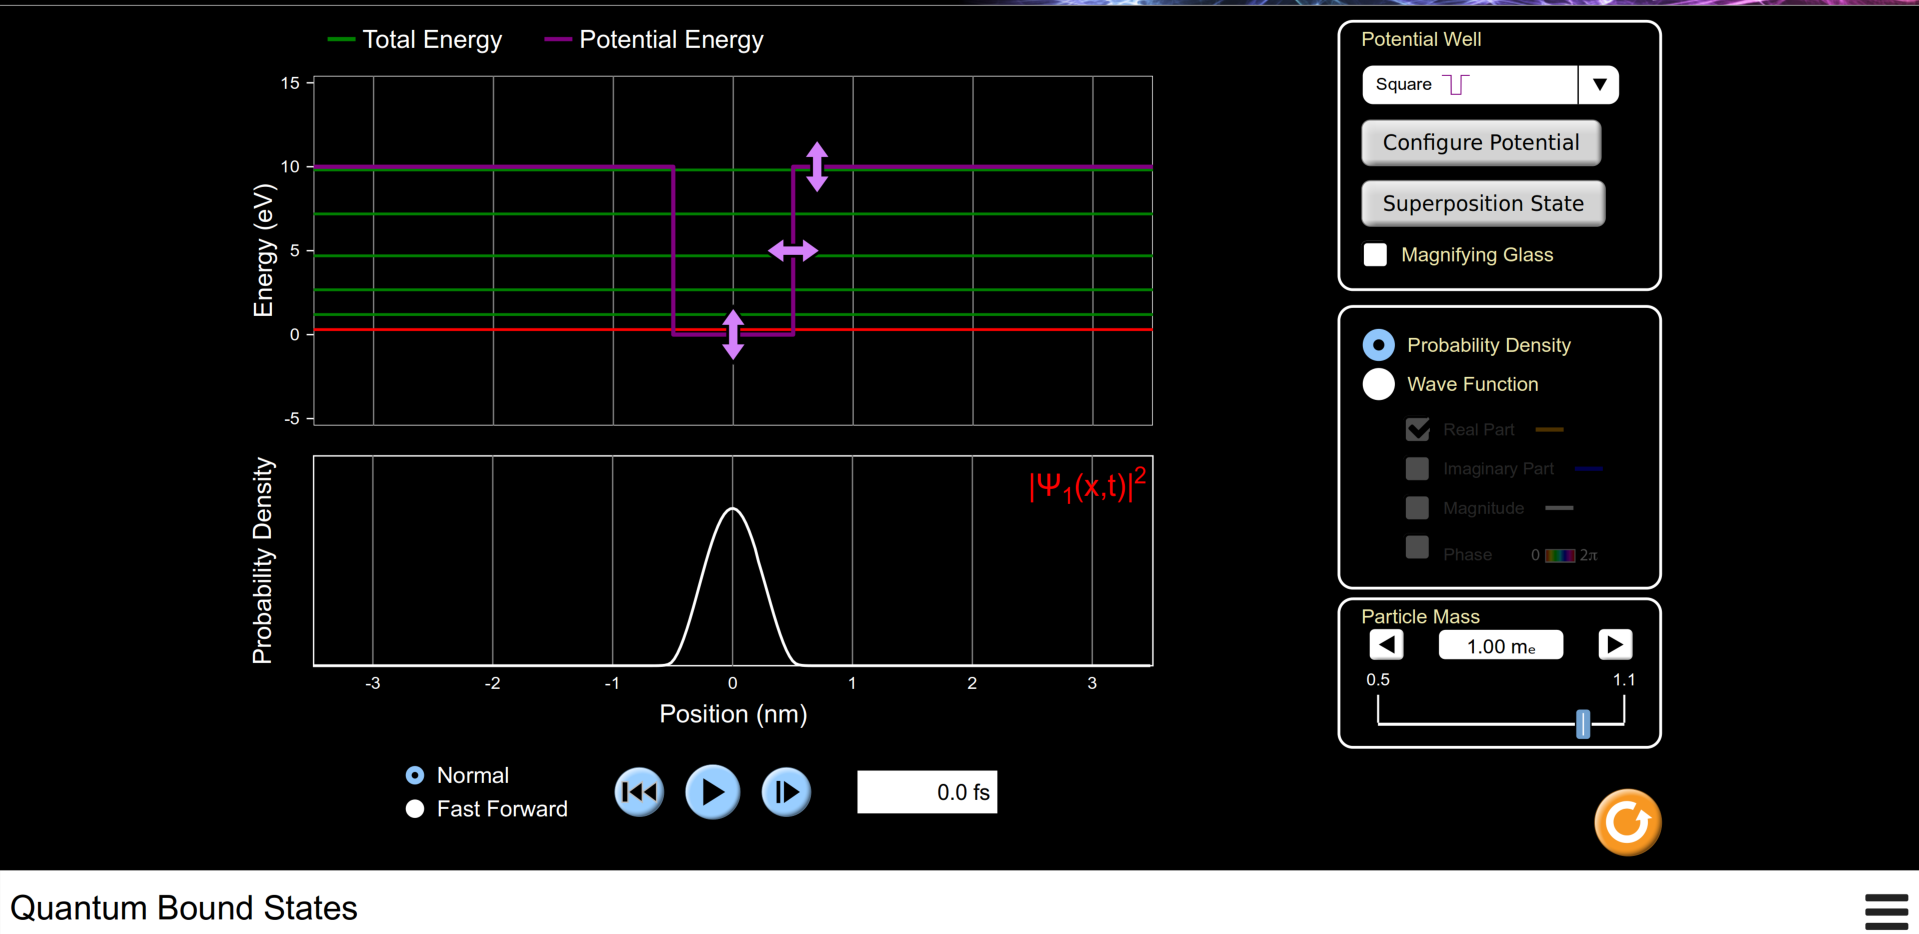
\includegraphics[width=\textwidth]{./img/initialscreenshot.png}
    \caption{Initial View}
\end{figure}

\begin{figure}[H]
    \centering
    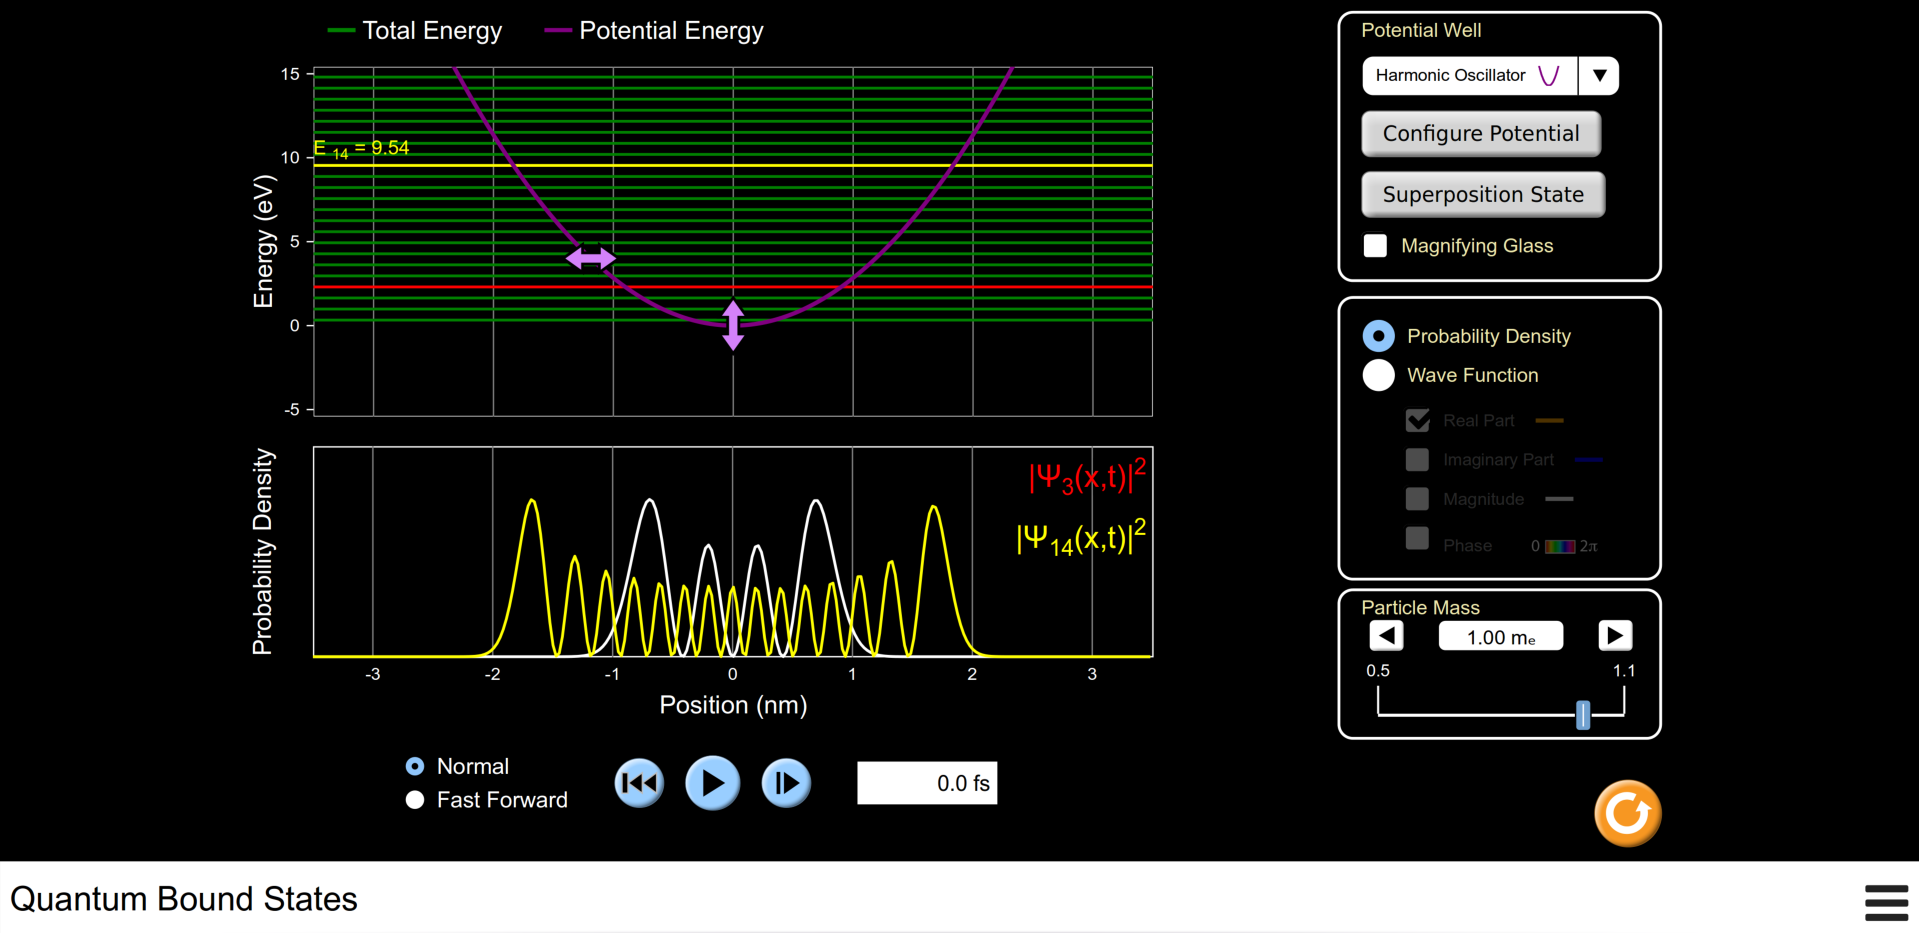
\includegraphics[width=\textwidth]{./img/harmonic_highlight.png}
    \caption{Harmonic Model}
\end{figure}

\begin{figure}[H]
    \centering
    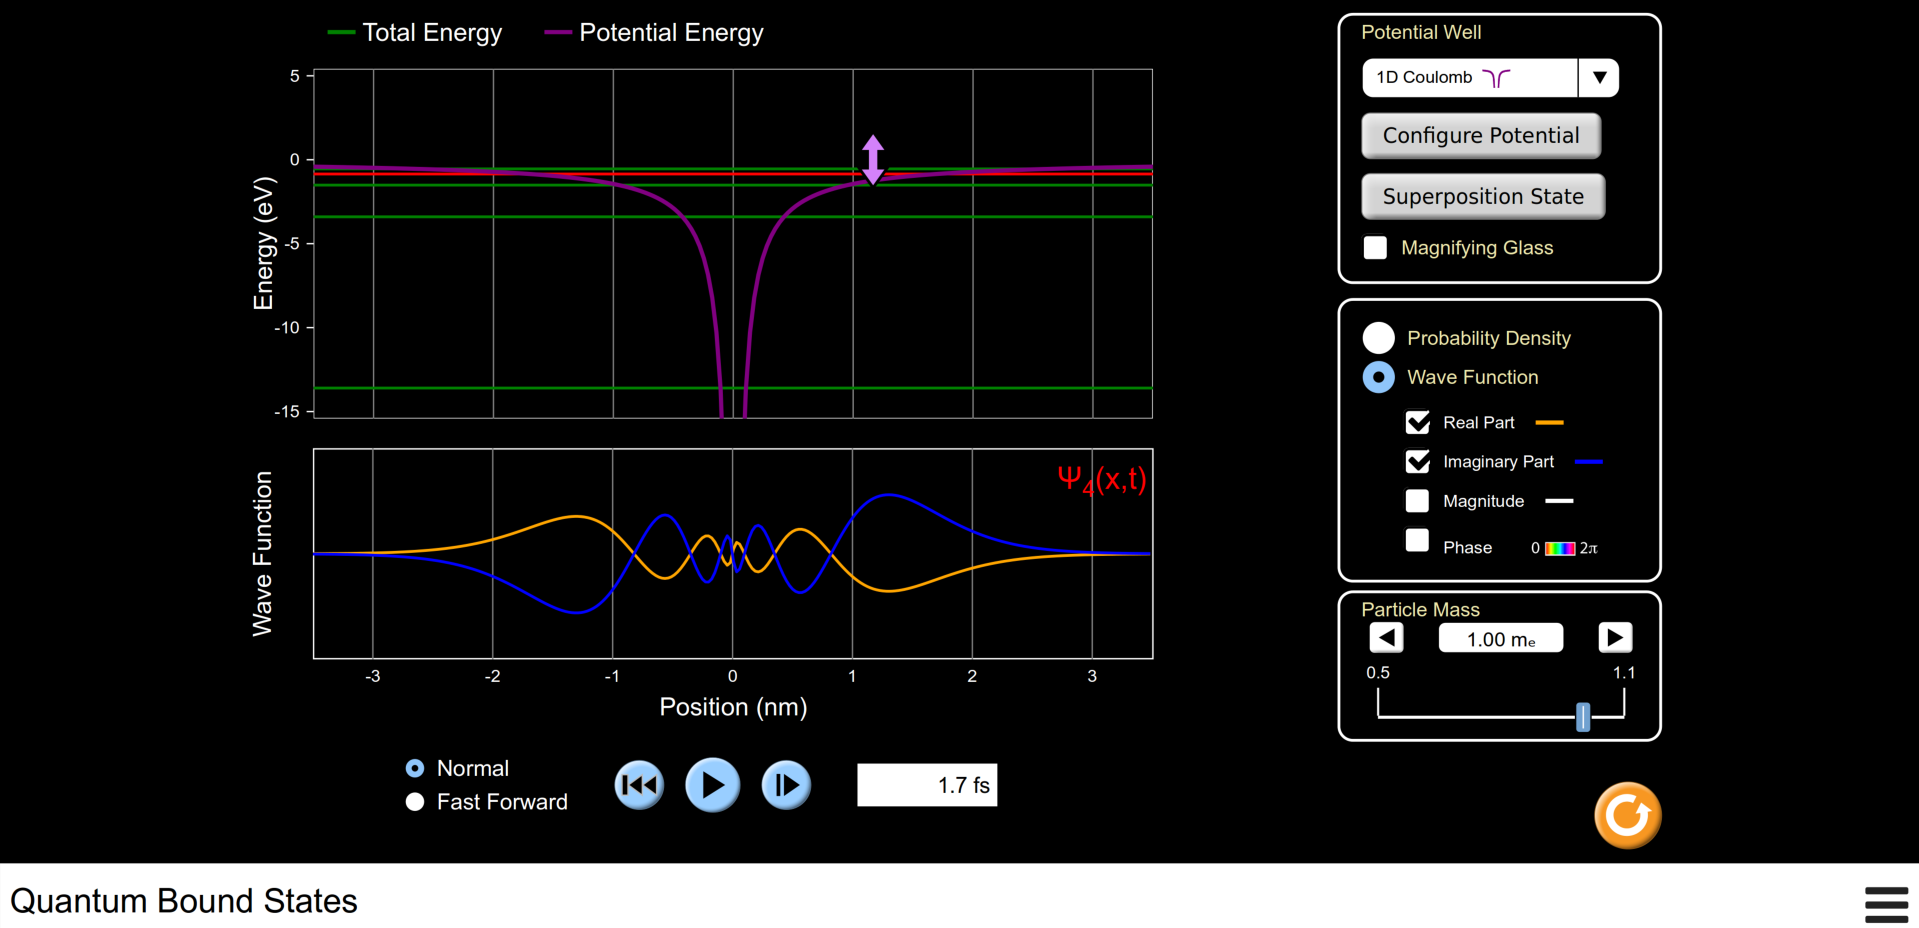
\includegraphics[width=\textwidth]{./img/wavefunction.png}
    \caption{Wave Function}
\end{figure}

The model maintains a unique reference to each potential well, so there is only one well of each
type in existence.  Each well has its own eigenstate cache and eigenvalue array, which change as the
properties governing the well shape change.  The model also maintains a reference to the unique
particle that is used in all calculations.  Specialized solver classes in the model calculate the
eigenstates, which are represented by 2D arrays of floating point numbers.  These eigenstates are
transformed by the main model class into the probability density function, the real wave function,
the imaginary wave function, and the magnitude of the wave function.  If the system is in a
superposition state, the model uses multiple eigenstates to calculate those functions.  The
superposition coefficients have their own class as part of the model, which handles all the updates
and notifications necessary for superposition states.

The view is based on a set of images created by PhET, which outline the updates to the UI from the
Java simulation.  The main section of the view contains a plot of the potential wells and the energy
eigenvalues, as well as a plot of the wave functions.  The potential wells are mutable; the user can
change their offset, height, width, and frequency, depending on the type of well being displayed.
The well types are square, asymmetric, 1D Coulomb, 3D Coulomb, and harmonic oscillator.  

Overlaid on each well is the set of energy lines, which each represent a different eigenstate.  The
lines are interactive; hovering over them makes their energy value appear, as well as a plot of
their associated wave function.  Clicking on them selects them as the current eigenstate.  They can
also be selected via the superposition state dialog box, which allows users to select multiple
eigenstates by setting their coefficients to a value other than zero.

The wave function plot switches between a plot of the probability density function and a plot of the
real and imaginary waves, plus their magnitude. The user can either select to display the wave
function or the probability density in a chart to the right of the wave function plot. If the wave
function is selected to be displayed, the user then has the further option of deciding which parts
of that wave function they want displayed. The user can select via check-box if they want to display
the real part, imaginary part, and/or magnitude.  Future work will allow users to view the phase
difference between the real and imaginary waves, as well.

Other control panels allow users to switch the potential well type, configure the properties
describing the potential well, and change the particle mass.  A set of controls at the bottom of the
simulation allows the user to start and stop the animation, take steps forward in time, and reset
time to zero.  When the animation is active, the waves oscillate, using the data managed by the
model.  Every time step, the model updates the arrays containing the wave function points, which
then notify the view to update itself with the new values.  Changing the parameters governing the
potential well, the particle mass, or the superposition state has the same effect.

\begin{figure}[H]
    \centering
    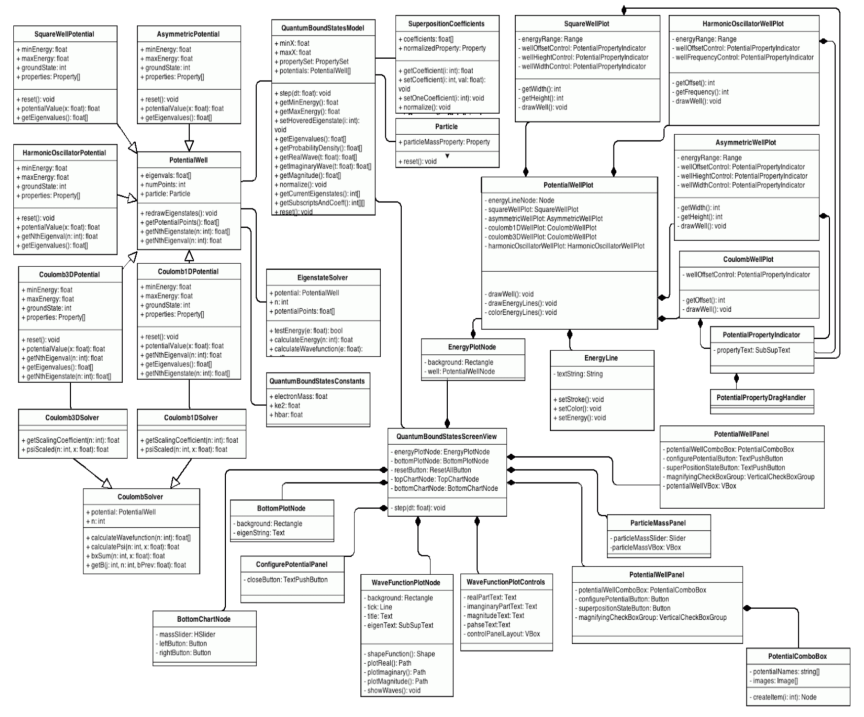
\includegraphics[width=\textwidth]{./img/finalclassdiagram.png}
    \caption{Final Class Diagram}
\end{figure}

\section{Design Patterns}

There are three main design patterns in our project. The first design pattern implemented is the
Observer pattern, implemented using PhET's {\ttfamily Property} class.  Each instance of the
{\ttfamily Property} class acts as a subject, and is unique among Subject classes in that it does
not directly maintain a list of Observer classes.  Instead, it maintains a list of functions.  The
main model class is a subclass of {\ttfamily PropertySet}, and thus generates a list of {\ttfamily
Properties}.  Those properties can be linked to any number of functions. Each time a property
changes, all of its linked functions are called.  So, instead of the one {\ttfamily update()}
function being called, the class keeps track of a list of functions to call every time it changes.
These functions are created by the observer classes. For the most part, the group of observers
consists of the view classes, although there are some classes in the model act as observers for some
cases.

The second design pattern our project implements is the Composite design pattern, which gives our
view its structure. The view classes (and in fact all drawable objects) inherit from PhET's
{\ttfamily Node} class, and they all can possess children of their own; this creates the tree
structure of the Composite pattern. While there is no specific leaf class, leaves can be understood
as childrenless nodes. Every class that inherits from {\ttfamily Node} can be drawn on the screen.

The third design pattern that we have used is the Model-View-Controller (MVC) architecture. Although
we did not use MVC exactly, as we do not have a specific set of controller classes, the fundamental
principles are present throughout the system. Most of the work that would be done by the controller
is in the view classes. These classes communicate with the model to update themselves, so there was
no real need for a set of controller classes.  The underlying code base, as created by PhET, does
include classes which primarily function as controllers, but we do not use any of them explicitly.

An additional design pattern that may have been useful is the Singleton pattern, as there should
only have ever been one instance of the particle, one instance of the superposition state
coefficients, and one instance of each potential well type.  However, Javascript makes that very
challenging, if not impossible, to implement.  The model therefore uses a jury-rigged version of
singleton, wherein it creates one instance of each class and then passes that instance to every
class that needs to use it.  It functions according to PhET's specifications, but it has the
potential to create problems if later developers do not realize that each instance should be a
singleton.

\section{Final System vs.\ Original Intent}

\begin{figure}[H]
    \centering
    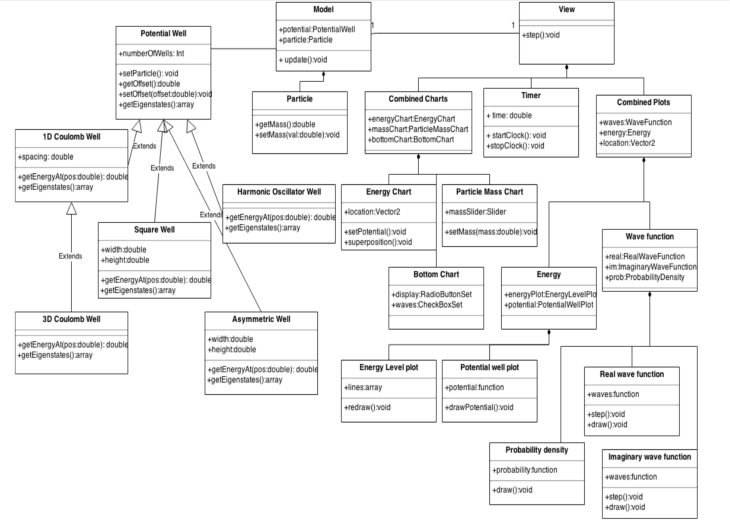
\includegraphics[width=\textwidth]{./img/initialclassdiagram.png}
    \caption{Initial Class Diagram}
\end{figure}

The specific structure of our classes changed significantly from the design presented in part 2,
although the functionality has not changed.  As we were porting the simulation directly from the
Java version, the functional requirements could not change.  But the class responsibilities and
hierarchy changed to better fit PhET's updated standards.  In the old class diagram, we had the
classes {\ttfamily Combined Charts} and {\ttfamily Combined Plots}. These two classes contained the
plots and control panels, respectively; they were the only two classes added as children of the main
view. The new design adds many more classes to the primary view class, following PhET's convention.
The class called {\ttfamily PotentialWellPlot} now draws the potential well and energy lines on the
top chart; and {\ttfamily WaveFunctionPlotNode} draws the wave function plots on the bottom chart.
Each are added to the main view class separately.  These same structural differences can be found
throughout the whole system.

The number of public variables and functions has also changed significantly.  In the model, that
number has increased; the views have no public variables and few public functions.  This is partly
because, in the system PhET created, a public function can't use a private function, so many
functions in the model which should have been private needed to be public, as they were necessary
for the public functions.  It's also because the model added a number of getter methods to more
easily access elements such as the superposition coefficients and the particle mass property.
However, the views do not need any public variables, and the only public functions they need are
ones that are called on them by other classes.  So only {\ttfamily EnergyLine} needed public
functions.

The model class structure changed as well: multiple solvers were added as their own classes, as
was a constants class and a class for the superposition state coefficients.  The solver classes
were added because their behavior was far too complex to include in the main model class; the
superposition coefficients became their own class for the same reason.  The latter started out
as a simple array of values, but became much more, as methods needed to be called on that
array, and it needed to have associated properties and dynamic behavior.  The constants class
was added to store the necessary physical constants, such as the mass of the electron, used in
numerous places.

Some of these changes were at the suggestion of Chris Malley, and others evolved naturally as
the project progressed.  Although the functionality was not affected, the changes made it
easier to add functionality and meet PhET's standards.  They should also make it easier to add
more features in the future.  We only implemented the first screen of {\ttfamily Quantum Bound
States}; the Java version contains two more screens.  Implementing those screens will be simpler
with the changes we made.

\section{Conclusion}

The project had many learning experiences that every member from the group can draw from in the
future. Before taking this course virtually all members of the group were strangers, which meant
that soon after the project began it became clear that communication was vital. Learning how to
effectively communicate ideas to new people is a skill that will be useful in industry and we have
all learned how important it is during the initial stages of this project. Once the project was
decided, the preparation and setup were critical parts of creating a successful simulation. This
planning stage included team meetings to decide how the project would be run, as well as the
construction of different diagrams illustrating how the project was going to be laid out. We
definitely learned that planning ahead in a project this size is important and that by following
common design patterns we could avoid many pitfalls. We designed the structure of the project
keeping in mind design techniques presented in class, and drawing from many resources including the
1994 book, \textit{Design Patterns: Elements of Reusable Object-Oriented Software}. This project
absolutely highlighted the fact that design patterns are important not only for keeping the project
streamlined and clean, but also for organizing the project to maintain productivity.

The best part of this project is the fact that we have now created a simulation that students will
be able to learn from for years to come. We hope that PhET is able to draw from and extend our
project in order to fully enable students that wish to learn from this simulation.
